\documentclass{article}
\usepackage{indentfirst}
\usepackage{blindtext}
\usepackage{graphicx}
\graphicspath{ {./images/} }

\title{Skills Assessment}
\author{Nathan Givens}
\date{November 8, 2019}

\setlength{\parindent}{4ex}

\begin{document}

  \maketitle

  \section*{UART Bus Decoding}

  UART bus decoding is a method of capturing communications over a UART bus and
  decoding the information sent between devices. Equipment often decodes the
  information into hexadecimal, but the equipment we have available can display
  the information in binary and ASCII as well. The procedure described in this
  document should apply to any of the oscilloscopes available in the senior
  design labs but was prepared using a Keysight MS0-X 3014T so there may be
  some subtle differences between models.

  \begin{figure}[h]
    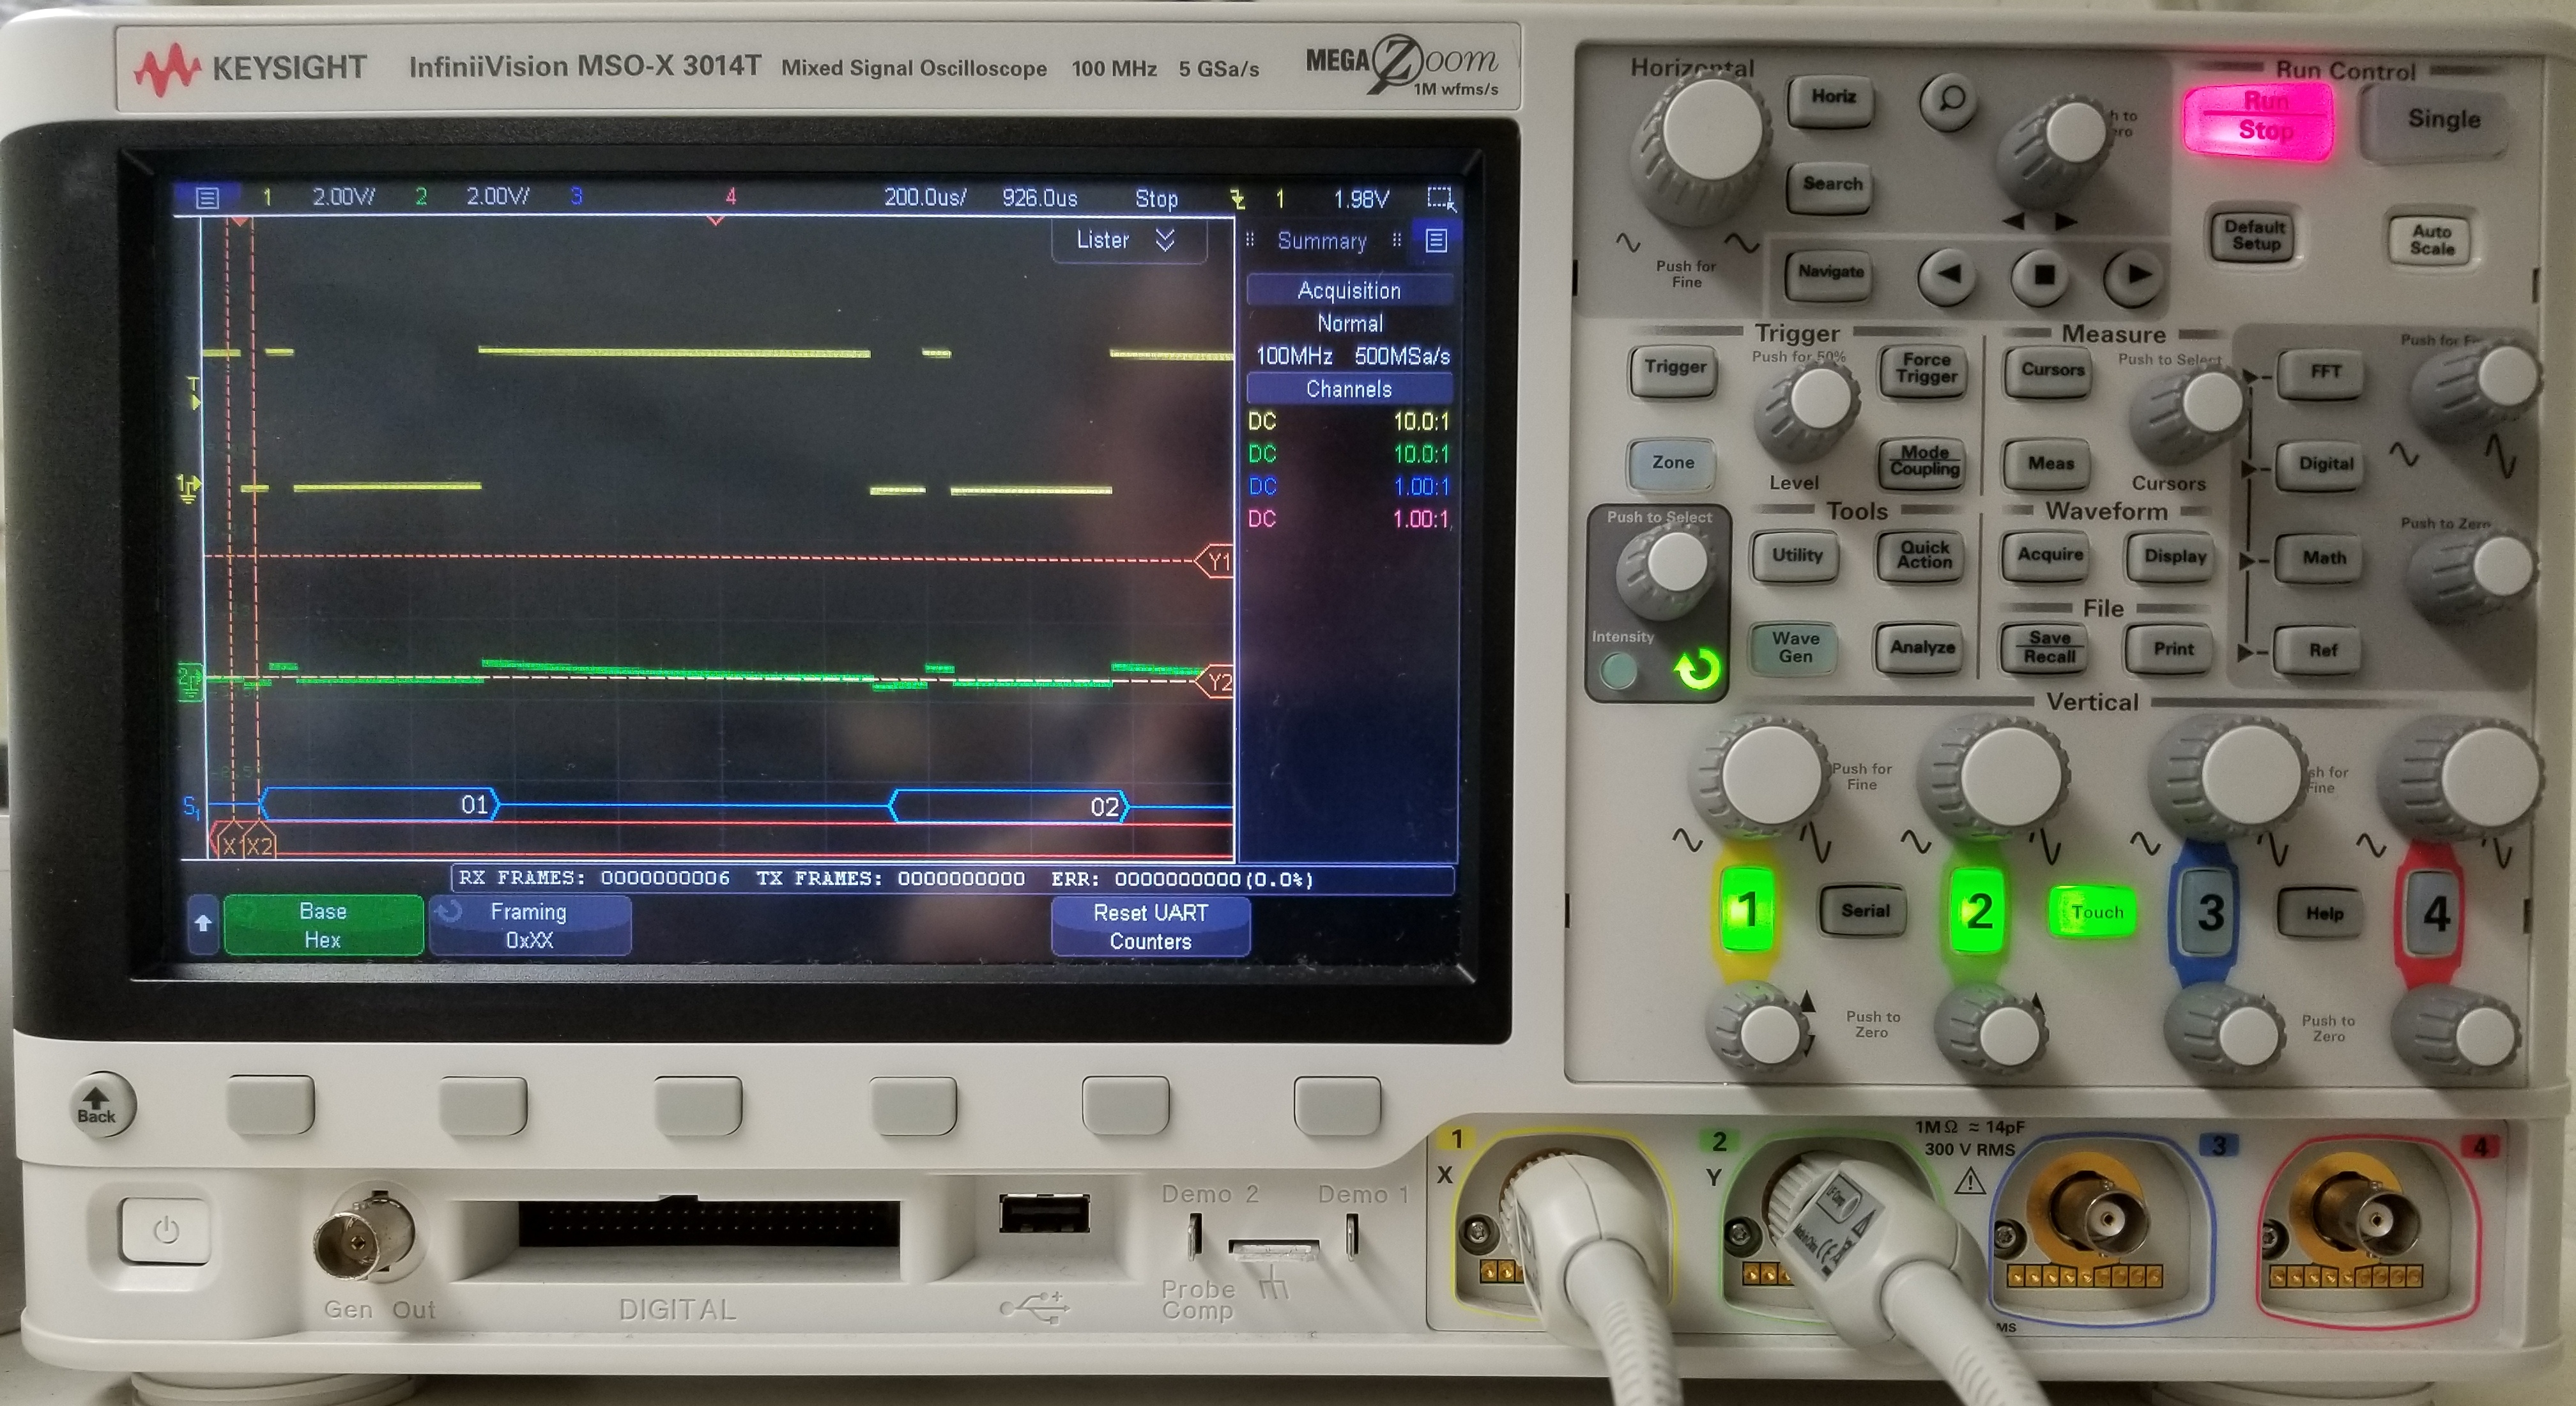
\includegraphics[width=\textwidth]{full_scope}
    \caption{An oscilloscope properly decoding data from a UART bus}
  \end{figure}

  Firstly, the oscilloscope must be turned on and the proper number of probes
  must be connected. For UART, two cables are needed to test two way
  asynchronous communications. If only one signal needs to be decoded, then only
  one cable needs to be connected to the oscilloscope.

  These oscilloscopes have a Serial button located between buttons 1 and 2
  for for probe configurations. This button opens the serial protocol decoding
  menu where settings can be changed to match the expected bus configurations.

  \begin{figure}[h]
    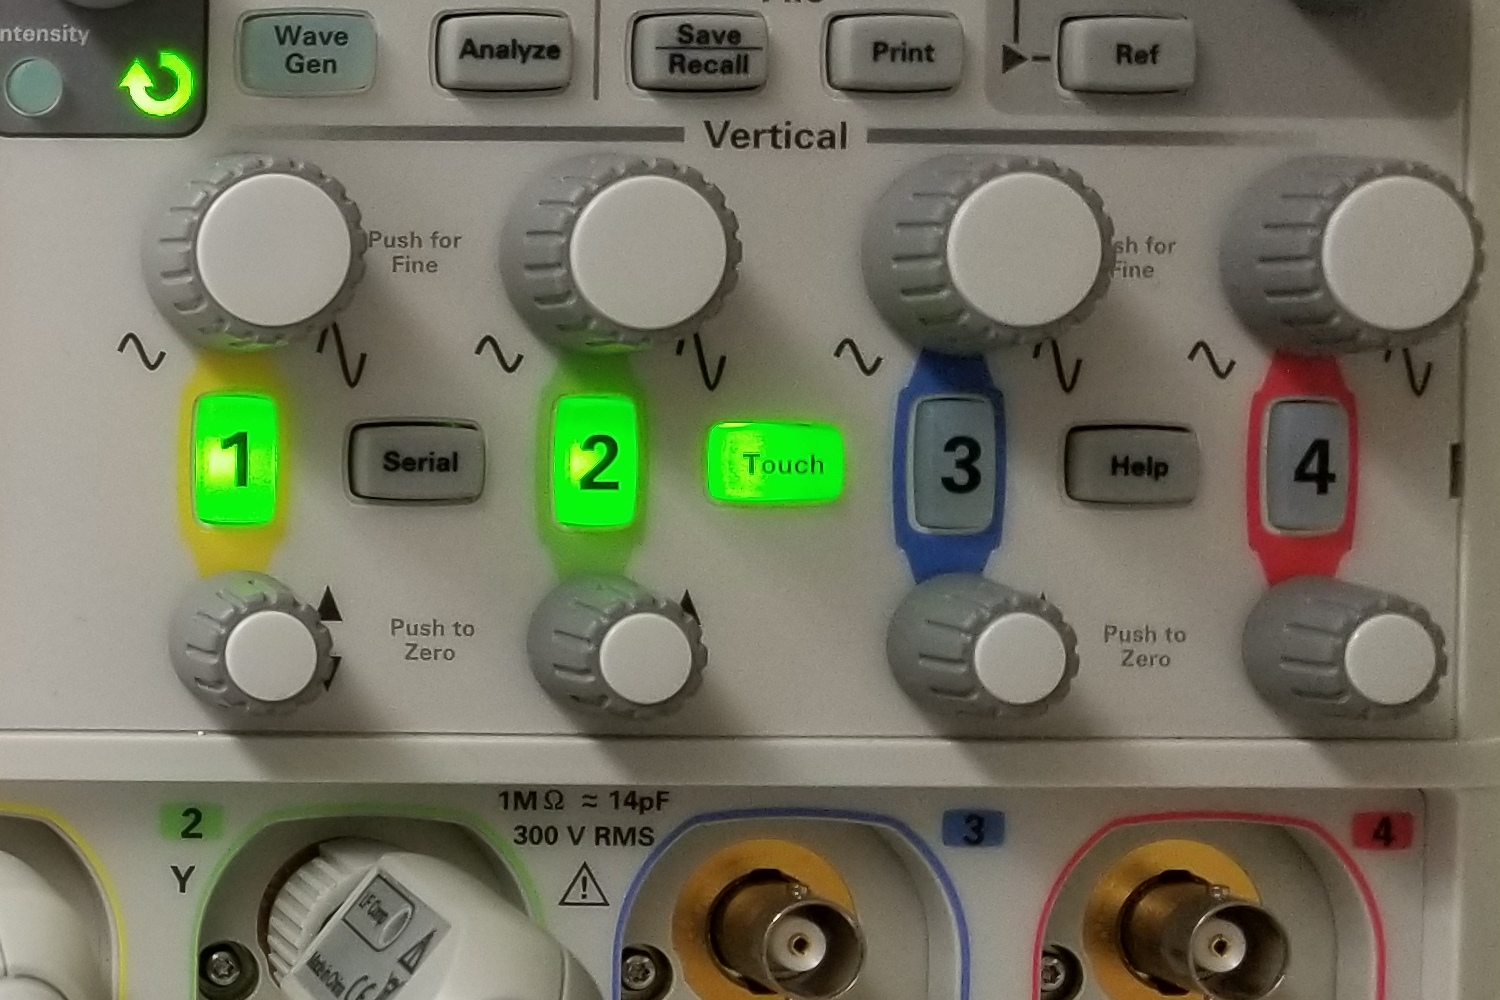
\includegraphics[width=50ex]{serial_button_scope}
    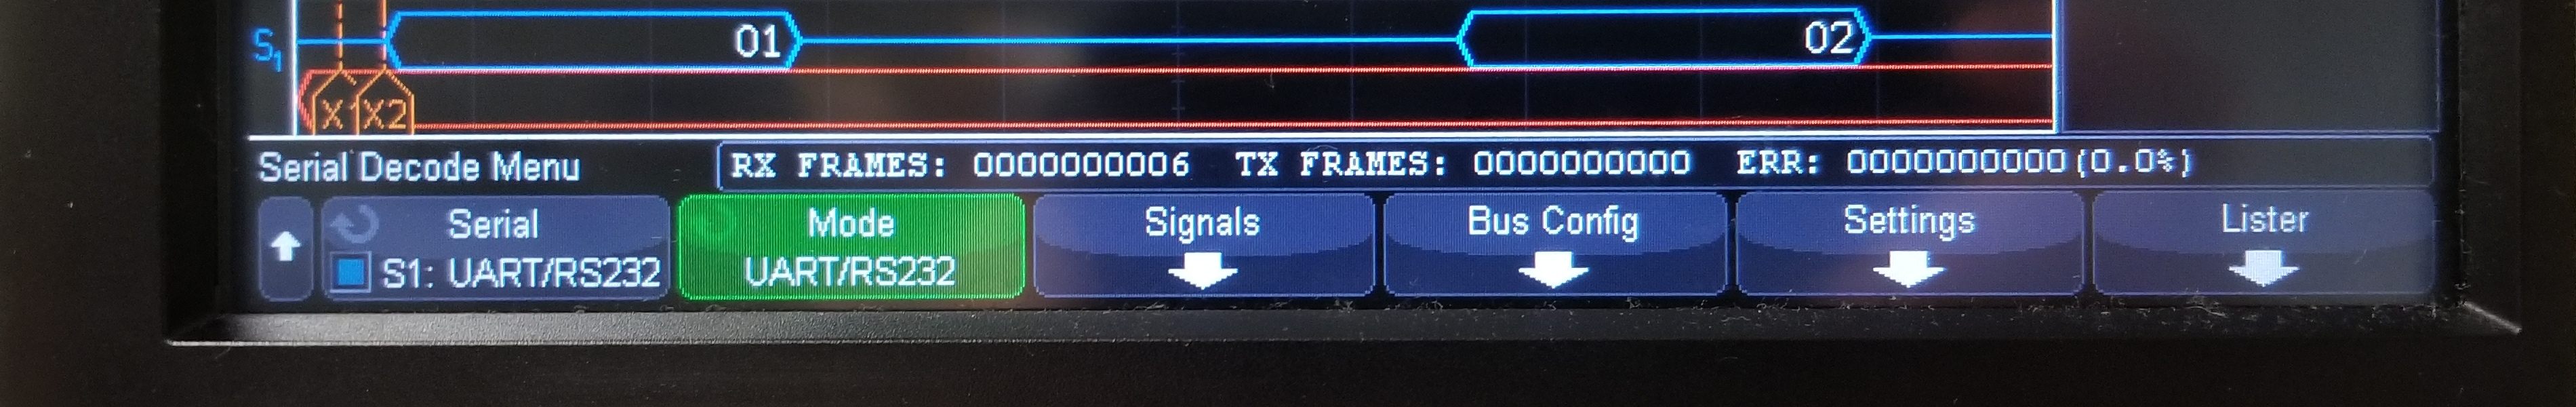
\includegraphics[width=\textwidth]{serial_decode_scope}
    \caption{Serial button and Serial Decode Menu}
  \end{figure}

\end{document}
